\documentclass[12pt]{article}
\usepackage{amsmath}
\usepackage{graphicx}
\usepackage{hyperref}
\usepackage{listings}
\usepackage{color}
\usepackage{pythonhighlight}

\title{Operating System Course Report - First Half of the Semester}
\author{B class}
\date{\today}

\begin{document}

\maketitle
\newpage

\tableofcontents
\newpage

\section{Introduction}
This report summarizes the topics covered during the first half of the Operating System course. It includes theoretical concepts, practical implementations, and assignments. The course focuses on the fundamentals of operating systems, including system architecture, process management, CPU scheduling, and deadlock handling.

\section{Course Overview}
\subsection{Objectives}
The main objectives of this course are:
\begin{itemize}
    \item To understand the basic components and architecture of a computer system.
    \item To learn process management, scheduling, and inter-process communication.
    \item To explore file systems, input/output management, and virtualization.
    \item To study the prevention and handling of deadlocks in operating systems.
\end{itemize}

\subsection{Course Structure}
The course is divided into two halves. This report focuses on the first half, which covers:
\begin{itemize}
    \item Basic Concepts and Components of Computer Systems
    \item System Performance and Metrics
    \item System Architecture of Computer Systems
    \item Process Description and Control
    \item Scheduling Algorithms
    \item Process Creation and Termination
    \item Introduction to Threads
    \item File Systems
    \item Input and Output Management
    \item Deadlock Introduction and Prevention
    \item User Interface Management
    \item Virtualization in Operating Systems
\end{itemize}

\section{Topics Covered}

\subsection{Basic Concepts and Components of Computer Systems}
This section explains the fundamental components that make up a computer system, including the CPU, memory, storage, and input/output devices.

\subsection{System Performance and Metrics}
This section introduces various system performance metrics used to measure the efficiency of a computer system, including throughput, response time, and utilization.

\subsection{System Architecture of Computer Systems}
Describes the architecture of modern computer systems, focusing on the interaction between hardware and the operating system.

\subsection{Process Description and Control}
Processes are a central concept in operating systems. This section covers:
\begin{itemize}
    \item Process states and state transitions
    \item Process control block (PCB)
    \item Context switching
\end{itemize}

\subsection{Scheduling Algorithms}
This section covers:
\begin{itemize}
    \item First-Come, First-Served (FCFS)
    \item Shortest Job Next (SJN)
    \item Round Robin (RR)
\end{itemize}
It explains how these algorithms are used to allocate CPU time to processes.

\subsection{Process Creation and Termination}
Details how processes are created and terminated by the operating system, including:
\begin{itemize}
    \item Process spawning
    \item Process termination conditions
\end{itemize}

\subsection{Introduction to Threads}
This section introduces the concept of threads and their relation to processes, covering:
\begin{itemize}
    \item Single-threaded vs. multi-threaded processes
    \item Benefits of multithreading
\end{itemize}

\begin{figure}[h]
    \centering
    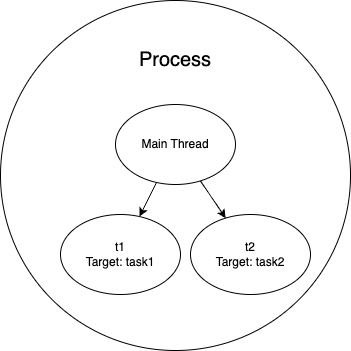
\includegraphics[width=0.5\textwidth]{/Users/khawaritzmi/Unhas/os_report_mid2024/b_class/asset/example.png}  % Sesuaikan nama file dan ukurannya
    \caption{Ini adalah gambar contoh dari multithreading.}
    \label{fig:contoh_gambar}
\end{figure}

Seperti yang terlihat pada Gambar \ref{fig:contoh_gambar}, inilah cara menambahkan gambar dengan keterangan.

\subsection{File Systems}
File systems provide a way for the operating system to store, retrieve, and manage data. This section explains:
\begin{itemize}
    \item File system structure
    \item File access methods
    \item Directory management
\end{itemize}

\subsection{Input and Output Management}
Input and output management is key for handling the interaction between the system and external devices. This section includes:
\begin{itemize}
    \item Device drivers
    \item I/O scheduling
\end{itemize}

\subsection{Deadlock Introduction and Prevention}
Explores the concept of deadlocks and methods for preventing them:
\begin{itemize}
    \item Deadlock conditions
    \item Deadlock prevention techniques
\end{itemize}

\subsection{User Interface Management}
This section discusses the role of the operating system in managing the user interface. Topics covered include:
\begin{itemize}
    \item Graphical User Interface (GUI)
    \item Command-Line Interface (CLI)
    \item Interaction between the user and the operating system
\end{itemize}

\subsection{Virtualization in Operating Systems}
    Virtualisasi memungkinkan beberapa sistem operasi berjalan secara bersamaan pada satu mesin fisik. Bagian ini akan membahasnya:
    
\subsubsection{Pengertian Virtualisasi Sistem Operasi}

\subsubsection{Jenis Jenis Virtualisasi pada Sistem Operasi}

\begin{figure}[h!]
    \centering
    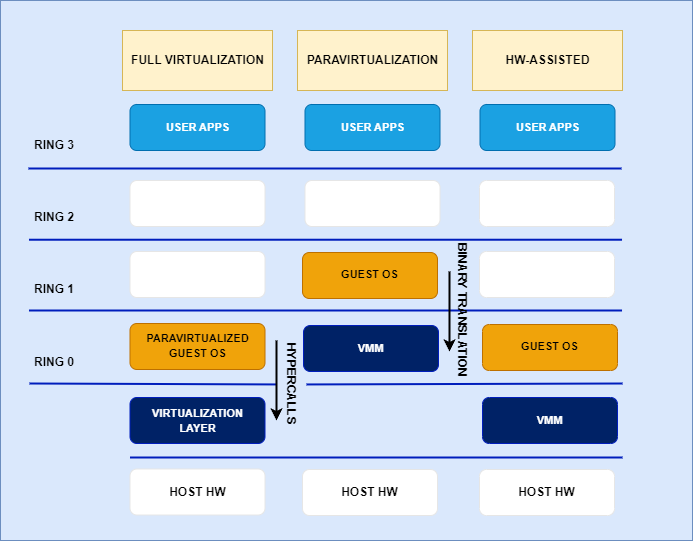
\includegraphics[width=0.8\textwidth]{assets/Asset_DS-Halaman-1.drawio.png}
    \caption{Type of Virtualization}
\end{figure}

\begin{enumerate}
    \item \textbf{Full Virtualization}
    \par Virtualisasi Penuh (\textit{Full Virtualization}), atau yang juga dikenal sebagai \textit{Native Virtualization}, adalah metode virtualisasi di mana mesin virtual (VM) digunakan untuk menjembatani sistem operasi tamu dengan perangkat keras fisik yang ada di bawahnya. Proses menjembatani ini sangat penting dalam teknik ini karena VM bertindak sebagai perantara antara sistem operasi tamu dan perangkat keras. Beberapa instruksi istimewa yang sensitif tidak dapat dijalankan langsung oleh sistem operasi tamu dan perlu diperangkap oleh \textit{hypervisor}, yang kemudian menangani instruksi tersebut, karena perangkat keras diakses melalui \textit{hypervisor}, bukan secara langsung oleh sistem operasi tamu.
    
    \par Kinerja Virtualisasi Penuh lebih cepat dibandingkan dengan metode emulasi perangkat keras, namun tetap lebih lambat dibandingkan dengan akses langsung ke perangkat keras fisik. Hal ini terjadi karena \textit{hypervisor} harus berfungsi sebagai media penghubung yang menyebabkan adanya \textit{overhead} dalam komunikasi antara sistem operasi tamu dan perangkat keras. Namun, keuntungan terbesar dari virtualisasi penuh adalah tidak memerlukan modifikasi pada sistem operasi tamu. Artinya, sistem operasi yang berjalan di atas virtualisasi penuh dapat berjalan sebagaimana adanya tanpa memerlukan perubahan atau penyesuaian khusus.
    
    \par Meski demikian, terdapat batasan dalam virtualisasi penuh, yaitu bahwa sistem operasi tamu harus kompatibel dengan perangkat keras yang ada di bawahnya. Beberapa jenis perangkat keras dapat menimbulkan masalah dalam virtualisasi penuh. Contohnya, beberapa instruksi sensitif tidak selalu bisa ditangkap oleh VM, yang berarti \textit{hypervisor} harus secara dinamis memindai instruksi tersebut menggunakan mode khusus pemerangkap untuk dapat menangani instruksi-instruksi tersebut. Ini menambah beban kerja \textit{hypervisor} dan dapat mempengaruhi performa sistem secara keseluruhan.
    
    \par Beberapa contoh implementasi virtualisasi penuh:
    \begin{itemize}
        \item \textbf{Contoh}
        \begin{itemize}
            \item \textit{VMware ESX Server}: Menggunakan \textit{hypervisor} tipe 1 yang berjalan langsung di perangkat keras, memungkinkan banyak mesin virtual tanpa modifikasi pada sistem operasi tamu.
    
            \item \textit{Microsoft Virtual Server}: Memungkinkan menjalankan sistem operasi tamu tanpa perubahan, meski kini lebih umum digunakan \textit{Hyper-V}.
        \end{itemize}
    \end{itemize}
    Untuk mengurangi \textit{overhead} ini, beberapa produsen perangkat keras seperti Intel dan AMD telah memperkenalkan teknologi yang mendukung virtualisasi secara langsung pada level perangkat keras, seperti Intel VT (\textit{Virtualization Technology}) dan AMD-V. Teknologi ini membantu mengurangi \textit{overhead} yang disebabkan oleh \textit{hypervisor} dengan memungkinkan sistem operasi tamu untuk berinteraksi lebih langsung dengan perangkat keras, sehingga meningkatkan efisiensi dan kinerja keseluruhan dari virtualisasi penuh.
    
    \par Dengan demikian, virtualisasi penuh menjadi salah satu pilihan yang sering digunakan dalam lingkungan server dan data center, karena kelebihannya dalam mendukung berbagai macam sistem operasi tanpa memerlukan perubahan pada kode sistem operasi tersebut, meskipun tetap ada beberapa batasan terkait performa dan kebutuhan perangkat keras khusus yang harus dipenuhi untuk memastikan virtualisasi berjalan secara optimal.

    \item \textbf{Para-Virtualization}
    \newline \textit{Para-virtualisasi} adalah teknik virtualisasi yang mirip dengan virtualisasi penuh, namun dengan pendekatan yang sedikit berbeda. Pada metode ini, \textit{hypervisor} tetap digunakan untuk berbagi akses ke perangkat keras, tetapi sistem operasi tamu perlu dimodifikasi agar lebih sadar akan proses virtualisasi. Pendekatan ini menghilangkan kebutuhan untuk melakukan \textit{rekompilasi} atau pemerangkapan instruksi, karena sistem operasi bekerja sama dengan \textit{hypervisor} dalam proses virtualisasi.

    \par Salah satu kelemahan utama dari \textit{para-virtualisasi} adalah bahwa sistem operasi tamu harus dimodifikasi agar kompatibel dengan lingkungan virtualisasi. Hal ini bisa menjadi kerugian bagi sistem operasi yang tidak siap untuk diubah atau dimodifikasi. 
    
    \par Beberapa contoh implementasi \textit{para-virtualisasi}:
    \begin{itemize}
        \item \textbf{Contoh}
        \begin{itemize}
            \item \textit{VMware ESXi: Hypervisor} tipe 1 yang memanfaatkan Intel VT dan AMD-V untuk efisiensi mesin virtual.

            \item \textit{KVM (Kernel-based Virtual Machine): Hypervisor} di Linux yang menggunakan ekstensi virtualisasi prosesor modern untuk kinerja optimal.
            
            \item \textit{Microsoft Hyper-V}: Platform virtualisasi yang memanfaatkan dukungan hardware untuk menjalankan mesin virtual dengan overhead minimal.
            
            \item \textit{Xen}: Meskipun menggunakan paravirtualisasi, \textit{Xen} juga memanfaatkan ekstensi hardware untuk meningkatkan performa.
        \end{itemize}
    \end{itemize}
    
    \par Keunggulan utama dari \textit{para-virtualisasi} adalah kemampuannya untuk memberikan performa yang mendekati sistem non-virtualisasi, karena \textit{overhead} yang lebih rendah dibandingkan dengan virtualisasi penuh. Mirip dengan virtualisasi penuh, beberapa sistem operasi dapat dijalankan secara bersamaan dalam lingkungan \textit{para-virtualisasi}. Namun, modifikasi pada sistem operasi menjadi persyaratan yang tidak dapat dihindari dalam metode ini.
    
    \par Cara kerja \textit{para-virtualisasi} dimulai dengan modifikasi pada sistem operasi tamu agar dapat berinteraksi secara langsung dengan \textit{hypervisor.} Dengan adanya \textit{Application Programming Interface (API)} yang disediakan oleh \textit{hypervisor}, sistem operasi dapat melakukan panggilan untuk mendapatkan akses ke sumber daya perangkat keras, seperti CPU dan memori, tanpa melalui proses penjebakan yang kompleks. Proses ini memungkinkan komunikasi yang lebih cepat dan efisien antara sistem operasi dan \textit{hypervisor}, sehingga mengurangi \textit{overhead} yang biasanya terdapat dalam virtualisasi penuh. Karena sistem operasi sudah "sadar" akan lingkungan virtualisasi, banyak instruksi sensitif dapat dijalankan dengan lebih langsung, sehingga memberikan kinerja yang lebih baik dibandingkan dengan metode virtualisasi lainnya.
    
    \item \textbf{Hardware-assisted Virtualization}
    \newline Virtualisasi Berbasis Hardware (\textit{Hardware-Assisted Virtualization}) mirip dengan Virtualisasi Penuh dan \textit{Para-virtualisasi}, tetapi memiliki perbedaan mendasar karena bergantung pada ekstensi hardware khusus yang dirancang untuk mengurangi \textit{overhead} dan meningkatkan performa. Teknik ini memanfaatkan fitur yang ada dalam prosesor modern, seperti \textit{Intel VT} (Vanderpool) dan \textit{AMD-V}(Pacifica), untuk menangani tugas yang biasanya menyebabkan kemacetan dalam virtualisasi berbasis perangkat lunak, terutama operasi I/O dan instruksi istimewa pada sistem operasi tamu.

    \par Beberapa contoh implementasi \textit{Hardware-Assisted Virtualization}:
    \begin{itemize}
        \item \textbf{Contoh}
        \begin{itemize}
            \item \textit{VMware ESXi}: Platform virtualisasi yang populer, menggunakan virtualisasi berbasis hardware untuk meningkatkan performa dan efisiensi.

            \item \textit{KVM (Kernel-based Virtual Machine)}: Solusi virtualisasi yang dibangun di atas kernel Linux, mendukung banyak mesin virtual dengan \textit{overhead} yang minimal.
            
            \item \textit{Microsoft Hyper-V}: Platform virtualisasi dari Microsoft yang memanfaatkan fitur virtualisasi berbasis hardware untuk menjalankan berbagai sistem operasi tamu secara efisien.
        \end{itemize}
    \end{itemize}

    \par Keunggulan utama dari virtualisasi berbasis hardware adalah kemampuannya untuk menjalankan sistem operasi tamu yang tidak dimodifikasi. Berbeda dengan \textit{Para-virtualisasi}, di mana sistem operasi tamu harus dimodifikasi agar bisa bekerja sama dengan \textit{hypervisor}, virtualisasi berbasis hardware memungkinkan sistem operasi tamu berinteraksi dengan perangkat keras seolah-olah ia berjalan langsung di mesin fisik. Perangkat keras memberikan dukungan untuk operasi terkawal dan terlindungi, sehingga meningkatkan efisiensi virtualisasi.
    
    \par Selain itu, virtualisasi berbasis hardware juga mengurangi kompleksitas dalam menangani instruksi sensitif. Dalam virtualisasi berbasis perangkat lunak, \textit{hypervisor} harus mencegat dan mengemulasikan instruksi terkawal, yang tidak efisien. Dengan fitur seperti \textit{Intel VT-x} dan \textit{AMD-V}, operasi sensitif ditangani langsung oleh prosesor, yang mempercepat manajemen mesin virtual dan eksekusi sistem operasi tamu.

    \item \textbf{OS-level Virtualization (Containerization)}
    
    \begin{figure}[h!]
        \centering 
        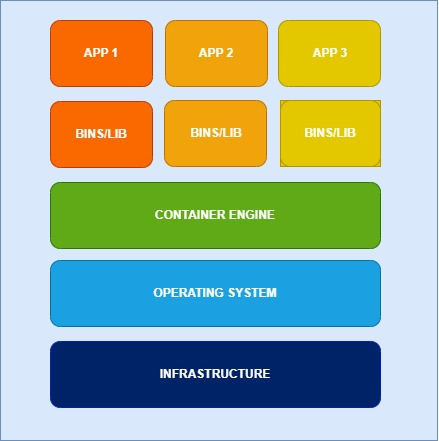
\includegraphics[width=0.8\textwidth]{assets/Asset_DS-Halaman-2.jpg}
        \caption{Containerization}
    \end{figure}
    
    \par \textit{OS-Level Virtualization}, atau lebih dikenal sebagai \textit{Containerization}, adalah teknologi yang memungkinkan pengembang untuk membungkus aplikasi beserta semua dependensinya ke dalam "kontainer" yang dapat dijalankan di berbagai lingkungan yang mendukung teknologi kontainer, seperti \textit{Docker} atau \textit{Kubernetes}. Kontainer ini berjalan di atas sistem operasi host yang sama, tetapi memberikan lingkungan runtime yang terisolasi dan konsisten untuk aplikasi. Hal ini memungkinkan pengembang untuk mengembangkan, menguji, dan menyebarluaskan aplikasi dengan lebih efisien dan konsisten.

    \par Keunggulan utama dari teknologi kontainerisasi adalah portabilitas dan efisiensi sumber daya. Kontainer dapat dengan mudah dipindahkan antar lingkungan, seperti dari pengembangan ke produksi, atau antara penyedia \textit{cloud} yang berbeda. Selain itu, kontainer lebih ringan dan menggunakan lebih sedikit sumber daya dibandingkan dengan mesin virtual tradisional. Namun, kontainer juga memiliki beberapa kerugian, seperti membutuhkan waktu lama untuk belajar dan memerlukan perhatian khusus dalam hal keamanan dan pengelolaan kompleksitas.
    
    \par Contoh yang paling populer dari teknologi kontainerisasi adalah \textit{Docker}. Dengan \textit{Docker}, pengembang dapat membuat versi aplikasi mereka dalam wadah yang dapat dijalankan di berbagai lingkungan. \textit{Docker} juga mendukung alat orkestrasi kontainer seperti \textit{Docker} \textit{Swarm} dan \textit{Kubernetes}, yang membantu mengelola klaster kontainer di beberapa host. Implementasi kontainerisasi biasanya dimulai dengan membuat image kontainer yang mencakup semua dependensi aplikasi, kemudian menjalankan image tersebut menggunakan \textit{Docker} atau alat lainnya.
\end{enumerate}

\par Jenis penerapan spesifik virtualisasi yang dibangun di atas dasar virtualisasi sistem operasi:

\begin{enumerate}
    \item \textbf{Desktop Virtualization}
    \begin{itemize}
        \item \textbf{Pengertian}: Proses menjalankan sistem operasi desktop dalam lingkungan virtual yang diakses dari jarak jauh.
        \item \textbf{Cara Kerja}: Sistem operasi desktop berjalan di server pusat, diakses melalui klien (\textit{thin client} atau komputer lain).
        \item \textbf{Keuntungan}: Akses dari mana saja dan manajemen terpusat untuk banyak pengguna.
    \end{itemize}

    \item \textbf{Network Virtualization}
    \begin{itemize}
        \item \textbf{Pengertian}: Pembuatan beberapa jaringan virtual di atas perangkat keras jaringan fisik.
        \item \textbf{Cara Kerja}: Setiap jaringan virtual terpisah seperti jaringan fisik.
        \item \textbf{Keuntungan}: Skalabilitas dan fleksibilitas dalam pengelolaan infrastruktur jaringan.
    \end{itemize}

    \item \textbf{Storage Virtualization}
    \begin{itemize}
        \item \textbf{Pengertian}: Menyatukan beberapa perangkat penyimpanan fisik menjadi satu sumber penyimpanan virtual.
        \item \textbf{Cara Kerja}: Data disimpan di beberapa perangkat tetapi disajikan seolah-olah berasal dari satu perangkat terpusat.
        \item \textbf{Keuntungan}: Meningkatkan fleksibilitas, manajemen, dan penggunaan penyimpanan.
    \end{itemize}

    \item \textbf{Application Virtualization}
    \begin{itemize}
        \item \textbf{Pengertian}: Teknologi yang memungkinkan aplikasi dijalankan di lingkungan virtual terpisah dari sistem operasi dasar.
        \item \textbf{Cara Kerja}: Aplikasi dibungkus dalam lingkungan virtual yang menyimpan semua dependensi dan konfigurasi.
        \item \textbf{Keuntungan}: Pengelolaan terpusat, keamanan yang ditingkatkan, portabilitas, dan efisiensi sumber daya.
    \end{itemize}
\end{enumerate}

\subsubsection{Komponen Virtualisasi Sistem Operasi}
\begin{enumerate}
    \item \textbf{Host Machine (Host OS)}:
        Sistem operasi fisik yang berjalan langsung di atas perangkat keras dan mengelola sumber daya seperti CPU, RAM, dan penyimpanan. Berfungsi sebagai platform untuk hypervisor.
    \begin{itemize}
        \item Contoh: Windows, Linux, macOS.
    \end{itemize}
    
    \item \textbf{Guest Machine (Guest OS)}:
        Sistem operasi virtual yang berjalan di atas mesin virtual (VM) dan diatur oleh \textit{hypervisor}. 
    \begin{itemize}
        \item Contoh: Linux, Windows.
    \end{itemize}
    
    \item \textbf{Hypervisor}:
    Perangkat lunak yang memungkinkan virtualisasi dan mengelola VM.
    \begin{itemize}
        \item Tipe 1 (\textit{Bare-metal}): Berjalan langsung di perangkat keras. Contoh: \textit{VMware ESXi, Hyper-V}.
        \item Tipe 2 (\textit{Hosted}): Berjalan di atas sistem operasi host. Contoh: \textit{VirtualBox, VMware Workstation}.
    \end{itemize}
    
    \item \textbf{Virtual Machine (VM)}:
    Lingkungan perangkat lunak yang dibuat oleh hypervisor untuk menjalankan guest OS secara terisolasi dari perangkat keras fisik.
\end{enumerate}

\subsubsection{Hypervisor dan Virtual Machines}
\subsubsection{Contoh Penerapan Virtualisasi pada Sistem Operasi}
\subsubsection{Kelebihan dan Kekurangan Virtualisasi pada Sistem Operasi}
\subsubsection{Kesimpulan}
    \par Virtualisasi sistem operasi telah menjadi fondasi penting dalam pengelolaan infrastruktur TI modern. Dengan memungkinkan pembuatan dan pengelolaan lingkungan virtual yang meniru perangkat keras fisik, teknologi ini memberikan efisiensi sumber daya yang signifikan, isolasi antara aplikasi, dan kemampuan skalabilitas yang tinggi. Teknik-teknik seperti\textit{ full virtualization, para-virtualization, dan containerization}, serta penggunaan \textit{hypervisor} tipe 1 dan tipe 2, memberikan fleksibilitas dalam pengelolaan berbagai sistem operasi dan aplikasi. Implementasi luas teknologi ini, yang mencakup solusi seperti \textit{VMware, VirtualBox, KVM, dan Docker,} menunjukkan kemampuannya dalam mendukung berbagai kebutuhan, mulai dari pengembangan dan pengujian perangkat lunak hingga manajemen infrastruktur TI yang kompleks. Dengan demikian, virtualisasi tidak hanya meningkatkan efisiensi operasional, tetapi juga memberikan kemudahan dalam pengelolaan sumber daya yang beragam, menjadikannya solusi yang sangat diperlukan dalam dunia TI yang terus berkembang.

    \begin{thebibliography}{9}
        \bibitem{umar2013}
        Umar, R., \& Fakultas Teknologi Industri Universitas Ahmad Dahlan Yogyakarta. (2013).\textit{ REVIEW TENTANG VIRTUALISASI.} JURNAL INFORMATIKA, 7(2), 775–777. 
        
        \bibitem{firmansyah2015}
        Firmansyah Adiputra. (2015). \textit{CONTAINER DAN DOCKER: TEKNIK VIRTUALISASI DALAM PENGELOLAAN BANYAK APLIKASI WEB.} \textit{Jurnal Ilmiah SimanteC}, 4(3), 167–169. Jl. Raya Telang, PO BOX 2 Kamal, Bangkalan. Retrieved September 27, 2024.
        
        \bibitem{knowledgehut2023}
        \textit{Operating System Virtualization – Types, Working, Benefits}. (2023, September 8). Retrieved from \url{https://www.knowledgehut.com/blog/cloud-computing/os-virtualization}
        
        \bibitem{geeksforgeeks2023}
        GeeksforGeeks. (2023, October 31). \textit{Types of server virtualization in computer network.} Retrieved from \url{https://www.geeksforgeeks.org/types-of-server-virtualization-in-computer-network/}
        
        \bibitem{hashemi2024}
        Hashemi-Pour, C., Brush, K., \& Kirsch, B. (2024, June 5). \textit{virtualization}. IT Operations. Retrieved from \url{https://www.techtarget.com/searchitoperations/definition/virtualization}
    \end{thebibliography}

\section{Assignments and Practical Work}
\subsection{Assignment 1: Process Scheduling}
Students were tasked with implementing various process scheduling algorithms (e.g., FCFS, SJN, and RR) and comparing their performance under different conditions.

\subsubsection{Group 1}
\subsubsection{Group 2}
\subsubsection{Group 3}
\subsubsection{Group 4}
\subsubsection{Group 5}
\subsubsection{Group 6}
\subsubsection{Group 7}
\subsubsection{Group 8}
\subsubsection{Group 9}
\subsubsection{Group 10}
\subsubsection{Group 11}
\subsubsection{Group 12}

\subsubsection{Group 13}
\begin{enumerate}
    \item Implementasi FCFS (First-Come, First-Served)
        \par Implementasikan algoritma penjadwalan FCFS. Buatlah fungsi yang menerima daftar proses (dengan waktu tiba dan waktu eksekusi) dan mengembalikan waktu penyelesaian, waktu tunggu, dan waktu respon untuk setiap proses. Gunakan daftar proses berikut sebagai contoh:
        \begin{table}[h!]
        \centering
        \begin{tabular}{|c|c|c|}
        \hline
        \textbf{Process ID} & \textbf{Arrival Time} & \textbf{Burst Time} \\ \hline
        1 & 0 & 4 \\ \hline
        2 & 1 & 2 \\ \hline
        3 & 2 & 1 \\ \hline
        \end{tabular}
        \caption{Process Scheduling Data}
        \end{table}
        
\begin{python}
def fcfs(processes):
    # Mengurutkan proses berdasarkan waktu kedatangan (arrival time)
    processes.sort(key=lambda x: x[1]) 
    completion_time = []
    waiting_time = []
    turnaround_time = []

    current_time = 0
    for process in processes:
        pid, arrival, burst = process
        if current_time < arrival: 
            current_time = arrival
        current_time += burst
        completion_time.append((pid, current_time))
        # Hitung waktu turnaround (selesai - tiba)
        turnaround_time.append((pid, current_time - arrival))
        # Hitung waktu tunggu (turnaround - burst)
        waiting_time.append((pid, current_time - arrival - burst))

    return completion_time, waiting_time, turnaround_time

processes = [(1, 0, 4), (2, 1, 2), (3, 2, 1)]
completion, waiting, turnaround = fcfs(processes)

print("FCFS:")
print("Completion Time:", completion)
print("Waiting Time:", waiting)
print("Turnaround Time:", turnaround)
\end{python}
        Output : 
        \par FCFS:
        \par Completion Time: [(1, 4), (2, 6), (3, 7)] 
        \par Waiting Time: [(1, 0), (2, 3), (3, 4)]
        \par Turnaround Time: [(1, 4), (2, 5), (3, 5)]
        
    \item Implementasi SJN (Shortest Job Next)
        \par  Implementasikan algoritma penjadwalan SJN. Buatlah fungsi yang menerima daftar proses (dengan waktu tiba dan waktu eksekusi) dan mengembalikan waktu penyelesaian, waktu tunggu, dan waktu respon untuk setiap proses. Gunakan daftar proses berikut sebagai contoh:
        \begin{table}[h!]
        \centering
        \begin{tabular}{|c|c|c|}
        \hline
        \textbf{Process ID} & \textbf{Arrival Time} & \textbf{Burst Time} \\ \hline
        1 & 0 & 4 \\ \hline
        2 & 1 & 2 \\ \hline
        3 & 2 & 1 \\ \hline
        \end{tabular}
        \caption{Process Scheduling Data}
        \end{table}
        
\begin{python}
def sjn(processes):
    # Mengurutkan proses berdasarkan waktu kedatangan
    processes.sort(key=lambda x: x[1]) 
    completion_time = []
    waiting_time = []
    turnaround_time = []
    
    current_time = 0
    while processes:
        # Memfilter proses yang telah tiba (waktu kedatangan <= waktu saat ini)
        available_processes = [p for p in processes if p[1] <= current_time]
        
        # Jika tidak ada proses yang siap, maju ke waktu kedatangan proses berikutnya
        if not available_processes:
            current_time = processes[0][1]
            continue
        
        # Memilih proses dengan waktu burst terpendek
        next_process = min(available_processes, key=lambda x: x[2])
        processes.remove(next_process)
        
        # Eksekusi proses terpilih
        pid, arrival, burst = next_process
        current_time += burst
        completion_time.append((pid, current_time))
        turnaround_time.append((pid, current_time - arrival))
        waiting_time.append((pid, current_time - arrival - burst))

    return completion_time, waiting_time, turnaround_time

processes = [(1, 0, 4), (2, 1, 2), (3, 2, 1)]
completion, waiting, turnaround = sjn(processes)

print("\nSJN (Shortest Job Next):")
print("Completion Time:", completion)
print("Waiting Time:", waiting)
print("Turnaround Time:", turnaround)
\end{python}
        Output : 
        \par SJN (Shortest Job Next):
        \par Completion Time: [(1, 4), (3, 5), (2, 7)]
        \par Waiting Time: [(1, 0), (3, 2), (2, 4)]
        \par Turnaround Time: [(1, 4), (3, 3), (2, 6)]
        
    \item Implementasi RR (Round Robin)
        \par  Implementasikan algoritma penjadwalan RR. Buatlah fungsi yang menerima daftar proses (dengan waktu tiba dan waktu eksekusi) serta kuota waktu, dan mengembalikan waktu penyelesaian, waktu tunggu, dan waktu respon untuk setiap proses. Gunakan daftar proses berikut sebagai contoh dan kuota waktu 2:
        \begin{table}[h!]
        \centering
        \begin{tabular}{|c|c|c|}
        \hline
        \textbf{Process ID} & \textbf{Arrival Time} & \textbf{Burst Time} \\ \hline
        1 & 0 & 4 \\ \hline
        2 & 1 & 2 \\ \hline
        3 & 2 & 1 \\ \hline
        \end{tabular}
        \caption{Process Scheduling Data}
        \end{table}
        
\begin{python}
from collections import deque

def rr(processes, quantum):
    processes.sort(key=lambda x: x[1]) 
    completion_time = {}
    waiting_time = {}
    turnaround_time = {}
    
    queue = deque()
    current_time = 0
    i = 0
    remaining_time = {pid: burst for pid, _, burst in processes}
    first_arrival_time = {pid: arrival for pid, arrival, burst in processes}

    while i < len(processes) or queue:
        # Memasukkan proses yang sudah datang ke dalam antrean
        while i < len(processes) and processes[i][1] <= current_time:
            queue.append(processes[i])
            i += 1
        
        if queue:
            pid, arrival, burst = queue.popleft()
            
            # Eksekusi proses selama quantum waktu atau sisa burst time
            execute_time = min(remaining_time[pid], quantum)
            remaining_time[pid] -= execute_time
            current_time += execute_time

            if remaining_time[pid] == 0:  # Proses selesai
                completion_time[pid] = current_time
            
            else:  # Proses belum selesai, masukkan kembali ke antrean
                queue.append((pid, arrival, remaining_time[pid]))
        
        else:
            # Jika tidak ada proses di antrean, pindah ke waktu kedatangan berikutnya
            if i < len(processes):
                current_time = processes[i][1]  

    # Menghitung waktu turnaround dan waktu tunggu untuk setiap proses
    for pid in completion_time:
        turnaround_time[pid] = completion_time[pid] - first_arrival_time[pid]
        waiting_time[pid] = turnaround_time[pid] - next(burst for p, arrival, burst in processes if p == pid)

    return completion_time, waiting_time, turnaround_time

processes = [(1, 0, 4), (2, 1, 2), (3, 2, 1)]
quantum = 2
completion, waiting, turnaround = rr(processes, quantum)

print("\nRR:")
print("Completion Time:", completion)
print("Waiting Time:", waiting)
print("Turnaround Time:", turnaround)
\end{python}
        Output : 
        \par RR:
        \par Completion Time: {1: 4, 2: 6, 3: 7}
        \par Waiting Time: {1: 0, 2: 3, 3: 4}
        \par Turnaround Time: {1: 4, 2: 5, 3: 5}
        
    \item Bandingkan Kinerja
        \par  Bandingkan kinerja algoritma penjadwalan FCFS, SJN, dan RR menggunakan daftar proses yang sama dan kuota waktu RR 2. Hitung waktu rata-rata untuk waktu tunggu masing-masing algoritma.
        \begin{table}[h!]
        \centering
        \begin{tabular}{|c|c|c|}
        \hline
        \textbf{Process ID} & \textbf{Arrival Time} & \textbf{Burst Time} \\ \hline
        1 & 0 & 4 \\ \hline
        2 & 1 & 2 \\ \hline
        3 & 2 & 1 \\ \hline
        \end{tabular}
        \caption{Process Scheduling Data}
        \end{table}
        
\begin{python}
def average_time(waiting_times):
    # Memastikan tidak terjadi pembagian dengan nol
    if len(waiting_times) == 0:
        return 0
    return sum([wt for pid, wt in waiting_times]) / len(waiting_times)

# Proses yang sama untuk semua algoritma
processes = [(1, 0, 4), (2, 1, 2), (3, 2, 1)]
quantum = 2

# Hitung kinerja setiap algoritma
fcfs_completion, fcfs_waiting, fcfs_turnaround = fcfs(processes)
sjn_completion, sjn_waiting, sjn_turnaround = sjn(processes)
rr_completion, rr_waiting, rr_turnaround = rr(processes, quantum)

# Hitung rata-rata waktu tunggu
avg_fcfs_waiting = average_time(fcfs_waiting)
avg_sjn_waiting = average_time(sjn_waiting)
avg_rr_waiting = average_time(rr_waiting)

print(f"\nRata-rata Waktu Tunggu:")
print(f"FCFS: {avg_fcfs_waiting}")
print(f"SJN: {avg_sjn_waiting}")
print(f"RR: {avg_rr_waiting}")
\end{python}
        Output : 
        \par Rata-rata Waktu Tunggu:
        \par FCFS: 2.3333333333333335
        \par SJN: 2.0
        \par RR: 0
\end{enumerate}

\subsection{Assignment 2: Deadlock Handling}
In this assignment, students were asked to simulate different deadlock scenarios and explore various prevention methods.

\subsection{Assignment 3: Multithreading and Amdahl's Law}
This assignment involved designing a multithreading scenario to solve a computationally intensive problem. Students then applied **Amdahl's Law** to calculate the theoretical speedup of the program as the number of threads increased.

\subsection{Assignment 4: Simple Command-Line Interface (CLI) for User Interface Management}
Students were tasked with creating a simple **CLI** for user interface management. The CLI should support basic commands such as file manipulation (creating, listing, and deleting files), process management, and system status reporting.

\subsection{Assignment 5: File System Access}
In this assignment, students implemented file system access routines, including:

\subsubsection{Group 1}
\subsubsection{Group 2}
\subsubsection{Group 3}
\subsubsection{Group 4}
\subsubsection{Group 5}
\subsubsection{Group 6}
\subsubsection{Group 7}
\subsubsection{Group 8}
\subsubsection{Group 9}
\subsubsection{Group 10}
\subsubsection{Group 11}
\subsubsection{Group 12}

\subsubsection{Group 13}
\begin{enumerate}
    \item File Creation and Deletion
        \par Buatlah fungsi Python yang dapat membuat file baru dengan nama yang diberikan dan menulis teks ke dalamnya. Juga, buat fungsi untuk menghapus file yang sudah ada.
\begin{python}
import os

# Membuat File Baru
def create_file():
    with open('new_file.txt', 'w') as file:
        file.write("Hello, World!")

create_file()

# Menghapus File
def delete_file():
    filename = 'new_file.txt'
    if os.path.exists(filename):
        os.remove(filename)

delete_file()
\end{python}
        
    \item Reading from and Writing to Files
        \par  Buatlah fungsi Python yang dapat membaca isi dari file yang diberikan dan menambahkan teks baru ke file tersebut.
\begin{python}
import os

# Membaca Isi File
def create_and_read_file():
    # Membuat file
    with open('read_file.txt', 'w') as file:
        file.write("This is a test file.")
    
    # Membaca file
    with open('read_file.txt', 'r') as file:
        content = file.read()
        print(content)

create_and_read_file()

# Menambahkan Konten ke File
def append_to_file():
    with open('read_file.txt', 'a') as file:
        file.write("Appending this line.\n")

append_to_file()
\end{python}
    \par Output :
    \par This is a test file.

    \item Navigating Directories and Managing File Permissions
        \par Ubah direktori kerja saat ini ke direktori \texttt{D:/Kuliah/SEMESTER-3/Sistem Operasi/os\_report\_mid2024} dan kembalikan isi dari direktori tersebut. Ubah izin akses file \texttt{read\_file.txt} menjadi hanya dapat dibaca oleh pemilik (mode: 0o400).

\begin{python}
import os

# Mengubah Direktori Kerja
def change_directory():
    try:
        os.chdir('D:\Kuliah\SEMESTER-3\Sistem Operasi\os_report_mid2024')
        return os.listdir()
    except FileNotFoundError:
        return None

directory_contents = change_directory()
print(directory_contents)

# Menambahkan Konten ke File
def append_to_file():
    with open('read_file.txt', 'a') as file:
        file.write("Appending this line.\n")

append_to_file()
\end{python}
    \par Output : 
    \par ['.git', '.gitignore', 'a\_class', 'b\_class', 'README.md']
\end{enumerate}

\section{Conclusion}
The first half of the course introduced core operating system concepts, including process management, scheduling, multithreading, and file system access. These topics provided a foundation for more advanced topics to be covered in the second half of the course.

\end{document}